%% AAMAS 2027 main-track submission (GTEP), built on the official AAMAS-2027 template
%% (aamas.cls, AAMAS_2027_sample.tex). Figures in figures/ are exported from the interactive
%% explainer (light theme, vector PDF). Earlier versions: archive_acmart/, archive_storyled/.
%% acmthm=false is a documented class option: it keeps one counter per theorem kind, which the
%% main paper and the supplement cross-reference.

%%%% For anonymized submission, use this
\documentclass[sigconf,anonymous,acmthm=false]{aamas}

%%%% For camera-ready, use this (and paste the block from authors_camera_ready.tex)
%\documentclass[sigconf,acmthm=false]{aamas}

\usepackage{balance} % for balancing columns on the final page

%%%%%%%%%%%%%%%%%%%%%%%%%%%%%%%%%%%%%%%%%%%%%%%%%%%%%%%%%%%%%%%%%%%%%%%%

%%% AAMAS-2027 copyright block (do not change!)

\makeatletter
\gdef\@copyrightpermission{
  \begin{minipage}{0.2\columnwidth}
   \href{https://creativecommons.org/licenses/by/4.0/}{
\includegraphics[width=0.90\textwidth]{by}}
  \end{minipage}\hfill
  \begin{minipage}{0.8\columnwidth}
   \href{https://creativecommons.org/licenses/by/4.0/}{This work is licensed under a Creative Commons Attribution International 4.0 License.}
  \end{minipage}
  \vspace{5pt}
}
\makeatother

\setcopyright{ifaamas}
\acmConference[AAMAS 2027]{Proc.\@ of the 26th International Conference
on Autonomous Agents and Multiagent Systems (AAMAS 2027)}{3--7 May 2027}{Hanoi, Vietnam}{M.~Baldoni, F.~Fang, W.~Yeoh, N.~Yorke-Smith (eds.)}
\copyrightyear{2027}
\acmYear{2027}
\acmDOI{}
%\acmPrice{}
\acmISBN{}

%%%%%%%%%%%%%%%%%%%%%%%%%%%%%%%%%%%%%%%%%%%%%%%%%%%%%%%%%%%%%%%%%%%%%%%%

%%% OpenReview submission number: printed on the first page in anonymous mode.
% Set the actual OpenReview number before submission: \acmSubmissionID{...}

\submissionType{Research Paper Track}

\usepackage{booktabs}
\usepackage{tabularx}
\usepackage{graphicx}
\usepackage{subcaption}
\usepackage[capitalise,nameinlink]{cleveref}

%% ---------- Theorem environments ----------
\theoremstyle{acmplain}
\newtheorem{theorem}{Theorem}
\newtheorem{lemma}{Lemma}
\newtheorem{proposition}{Proposition}
\newtheorem{corollary}{Corollary}
\theoremstyle{acmdefinition}
\newtheorem{definition}{Definition}
\emergencystretch=1.5em

%% ---------- Notation ----------
\newcommand{\E}{\mathbb{E}}
\newcommand{\Pb}{\mathbb{P}}
\newcommand{\TV}{\mathrm{TV}}
\newcommand{\dH}{d_{\mathrm{H}}}
\newcommand{\Kflat}{K_{\mathrm{flat}}}
\newcommand{\dmin}{d_{\min}}
\newcommand{\shat}{\hat{s}}
\newcommand{\cube}{\{0,1\}}
\newcommand{\A}{\textsf{Alpha}}
\newcommand{\B}{\textsf{Beta}}
\newcommand{\G}{\textsf{Gamma}}

\begin{document}

\title[How Much Memory Does Accountability Cost?]{How Much Memory Does Accountability Cost?}
\subtitle{Incentives and Reconstruction from Bounded Multi-Agent Records}

\begin{abstract}
What must a compressed record retain to support incentives for a team? We study a principal
who commits to an encoder of observable outcomes into $K$ labels and to bounded payments
that depend only on the retained label. A minimax characterisation eliminates the payment
rule and gives the largest effort cost supportable in dominant strategies. With independent
noisy binary outcomes, even Nash implementation requires the squared incentive margins to
sum to at most a constant times record entropy. For fixed noise parameters and positive
effort cost, memory therefore grows linearly with team size. One threshold bit per block
gives a constructive upper bound; its asymptotic per-agent rate is within $\pi\ln2$ of the
lower bound as effort cost tends to zero. Under a fixed total payment, the margin is instead
bounded by how well the record distinguishes individual deviators; permutation-invariant
outcome records cannot sustain positive effort. Deferred settlement can improve incentives
without increasing the maximum payment per task when agents receive no interim feedback.
For exact outcomes we derive the one-bit reconstruction--incentive frontier and identify
2-domination as the threshold for reconstruction-optimal accountability in the dominating-code
regime, with certified unrestricted thresholds in small dimensions. A model-written review
study illustrates attribution loss after removing names and shuffling reports, without
establishing strategic implementation. The results distinguish preserving task information
from preserving the evidence on which incentives depend.
\end{abstract}

\keywords{Moral hazard in teams; contract design; budget balance; information structures; mechanism design; repeated games; accountability; compressed records; LLM multi-agent systems}

\maketitle

%% =====================================================================
\section{Introduction}\label{sec:intro}
%% =====================================================================

Consider a principal commissioning a code review from three independently operated agents:
\A{} checks API changes, \B{} tests, and \G{} security. Their operators incur a cost for
careful work and receive a reward based on the evidence retained after review. Suppose the
principal can retain only a bounded record and settlement cannot consult the original traces.
A useful summary of the findings may then omit the evidence needed to reward an individual
reviewer. Which records preserve both functions?

Context compaction motivates an explicit retention constraint: reconstruction and
settlement see only the retained record. Strategic agents are service providers or their
operators, who bear effort costs and value rewards. Reconstruction recovers an outcome
profile under Hamming loss; accountability preserves effort's effect on expected bounded
payment. Accuracy alone need not preserve incentives (\cref{fig:pipeline}).

\begin{figure*}[t]
\centering
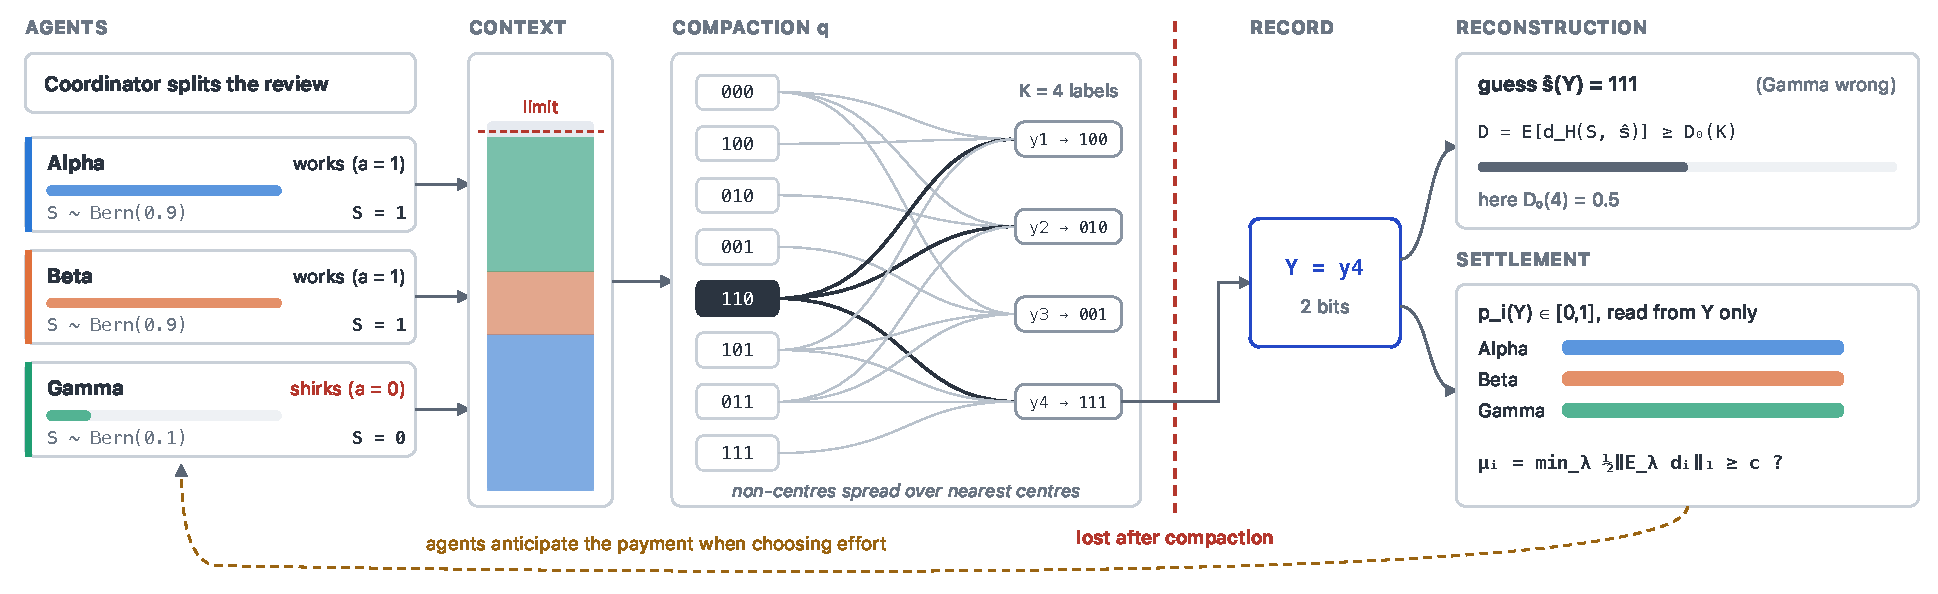
\includegraphics[width=\textwidth,page=1]{figures/pipeline_v3.pdf}
\caption{The object of study on the running example. Three agents choose effort; \A{} and \B{}
work and \G{} shirks; the displayed noisy outcome realisation is $S=110$. The record $q$
maps profiles to $K=4$ labels; the flat record of \cref{lem:suff} spreads $110$ over its three
neighbouring centres. Only the label survives. A reconstruction rule and a bounded payment rule
both read it, and agents anticipate the payment when choosing effort.}
\Description{Flow diagram in five columns. Agents: a coordinator and three agents, Alpha and
Beta working and Gamma shirking, with outcome bits 1, 1 and 0. Context: a context window
filled past its limit. Compaction: eight effort profiles from 000 to 111 connected by curves
to four labels; profile 110 is highlighted and connects to three labels. A red dashed line
marks what is lost after compaction. Record: the surviving label y4, two bits. Reconstruction
and settlement: a guess of who worked with its error, and bounded payments to each agent with
the margin formula. A dashed line returns from settlement to the agents.}
\label{fig:pipeline}
\end{figure*}

Moral hazard in teams~\cite{holmstrom1982teams} and algorithmic
contracts~\cite{babaioff2006combinatorial,castiglioni2023multiagent,dutting2025multiagent,dutting2025combinatorial,goel2024weighted,dutting2024survey}
connect observable outcomes to incentives. Bounded-payment contracts~\cite{kadanswinkels2008}
study limits on rewards for a given information structure; optimal monitoring
design~\cite{georgiadisszentes2020} also makes information acquisition endogenous.
Our constraint concerns a shared, finite retained alphabet, serving multiple agents'
incentives and reconstruction simultaneously. LLM failure
attribution~\cite{zhang2025which,zhang2025agentracer,cemri2025fail,chen2026elephant} and trace
compression~\cite{hong2026trace,lin2026tracer} motivate evaluating these objectives separately.
We ask: \emph{which outcome records fit a given information budget and still support effort?}

The contributions are three connected results.
\begin{enumerate}
\item \textbf{The memory price of incentives.} A minimax reduction characterises a fixed
record's dominant-strategy margin (\cref{thm:elim}). For independent noisy outcomes,
\cref{thm:noisy,thm:tight} give finite-size lower and constructive upper bounds for Nash
implementation. At fixed noise parameters, the achievable per-agent memory rate is
$\Theta(c^2)$ in the small-cost, large-team regime, with asymptotic ratio $\pi\ln2$ between
the block construction and the lower bound.
\item \textbf{Attribution and settlement constraints.} Under fixed-total payments,
\cref{thm:bb} bounds incentives by distinguishability among individual deviators, ruling out
permutation-invariant outcome records. Separate results characterise minimum expected
payments and show how deferred settlement helps without interim feedback
(\cref{prop:cost,thm:deferred}). These statements distinguish detection, attribution, and timing.
\item \textbf{Reconstruction without an incentive penalty.} With exact outcomes,
\cref{thm:onebit} gives the one-bit frontier. \Cref{thm:flat} identifies the 2-domination
threshold within the dominating-code regime and supplies a universal construction. The
supplement gives small-dimension certificates and a nearest-centre characterisation for
every full-support prior. Equal-error records can have margins $1/2$ and zero
(\cref{tab:mech}).
\end{enumerate}
The proofs are accompanied by executable checks and explicit code certificates. The
model-written review study is an attribution illustration, not evidence that the agents
respond strategically to payments. \Cref{tab:settings} separates the assumptions behind the
main results; the supplement documents computation and the study's limitations.

%% =====================================================================
\section{Model and the Settlement Game}\label{sec:model}
%% =====================================================================

\paragraph{Exact outcomes and records.} We first define the exact-outcome benchmark. A team of $n$ agents produces a profile
$S\in\cube^n$, where $S_i=1$ means agent $i$ did its work; we write profiles in agent order,
so with agents \A, \B, \G, the profile $011$ means only \A{} shirked. The uniform prior on $S$ evaluates reconstruction in this benchmark; it is not an equilibrium
assumption. In \cref{sec:noisy}, effort is hidden and $S$ instead denotes noisy outcomes,
with an action-dependent distribution. A \emph{record} of size $K$
is a stochastic encoder $q:\cube^n\to\Delta([K])$ with $q[s,y]=\Pb(Y=y\mid S=s)$. The label
$Y$ is everything that persists: the encoder's coins are not retained, and any seed, receipt
or identifier kept outside the record counts toward $K$, since one private bit per agent
beside a single shared label would evade the intended information budget. We report
$\log_2K$ as log-cardinality in bits; a fixed-length binary representation requires
$\lceil\log_2K\rceil$ bits. The known encoder and payment rules are not part of this
per-instance budget.

\paragraph{Reconstruction.} A rule $\shat:[K]\to\cube^n$ has expected Hamming error
$D(q,\shat)=\E[\dH(S,\shat(Y))]$, and $D_0(K)=\min_{q,\shat}D(q,\shat)$ is the $K$-median
value of the cube.

\begin{table}[t]
\caption{Settings and guarantees. DS: dominant strategies; Nash: all-work is a Nash equilibrium.
Unless specified, each payment lies in $[0,1]$.}
\label{tab:settings}
\footnotesize
\begin{tabularx}{\columnwidth}{@{}lXX@{}}
\toprule
result & observations & guarantee / restriction\\
\midrule
Theorems 2--3 & independent noisy outcomes & Nash; no fixed total\\
Theorem 4 & noisy outcomes & Nash; fixed total payment\\
Theorem 5 & repeated noisy outcomes & no interim feedback; payment in $[0,T]$\\
Theorems 6--7 & exact outcomes; uniform prior & DS and optimal reconstruction\\
\bottomrule
\end{tabularx}
\end{table}

\paragraph{Payment and the margin.} Agent $i$ is paid by a bounded decoder $p_i\in[0,1]^K$
that also sees only $Y$. The \emph{deviation vector} of agent $i$ at teammate profile
$s_{-i}$ is $d_i(s_{-i})[y]=q[(1,s_{-i}),y]-q[(0,s_{-i}),y]$, the change in the label
distribution caused by $i$ alone. The record \emph{implements margin} $\mu$ if bounded
decoders exist with
\begin{equation}\label{eq:M}\tag{M}
\langle p_i,d_i(s_{-i})\rangle\ge\mu\quad\text{for every } i \text{ and every } s_{-i}.
\end{equation}
The left side is $i$'s expected pay when working minus when shirking, with teammates fixed,
so the margin is the extra pay an agent is guaranteed for working, whatever the others do.
\Cref{tab:alpha} computes it for \A{} under the success-count record at $n=3$.

\begin{table}[t]
\caption{\A's margin under the success-count record ($n=3$) with the optimal bounded
payment, $1/3$ per recorded success. Every teammate profile gives the same gap, so the margin
is $1/3$, although \A's deviation always changes the count.}
\label{tab:alpha}
\footnotesize
\begin{tabular}{@{}lccc@{}}
\toprule
teammates (\B, \G) & pay, \A{} works & pay, \A{} shirks & gap\\
\midrule
$00$ & 0.33 & 0.00 & 0.33\\
$10$ or $01$ & 0.67 & 0.33 & 0.33\\
$11$ & 1.00 & 0.67 & 0.33\\
\bottomrule
\end{tabular}
\end{table}

\begin{definition}[Settlement game]\label{def:game}
Fix a record $q$. Each agent $i$ chooses $a_i\in\cube$ at cost $c_i\ge0$; the profile draws
$Y\sim q[a,\cdot]$; agent $i$ is paid $p_i(Y)\in[0,1]$ and gets $\E[p_i(Y)]-c_ia_i$. A payment
rule \emph{implements in dominant strategies} effort by $i$ if working is a best response whatever the
teammates do: $\langle p_i,d_i(s_{-i})\rangle\ge c_i$ for every $s_{-i}$.
\end{definition}

\begin{proposition}[The margin is a price]\label{prop:threshold}
Let $\mu_i(q)$ be the largest margin $q$ implements for agent $i$. Effort costing $c_i$ is
implementable in dominant strategies from $q$ by bounded payments if and only if $\mu_i(q)\ge c_i$. When
this holds for every agent, all-work is a dominant-strategy equilibrium with automatic participation,
and no payment rule with the same $[0,1]$ bounds and access only to $Y$ does better.
\end{proposition}
\begin{proof}
The first claim is \cref{def:game} at $\mu=c_i$. Participation holds since
$\E[p_i\mid a_i=1]\ge c_i+\E[p_i\mid a_i=0]\ge c_i$. Any bounded transfer that is a function
of $Y$ becomes a decoder in $[0,1]^K$ after an affine rescaling, which scales gaps and costs
together.
\end{proof}

The object of study is the least error at a required margin,
$D^*(K,\mu)=\min\{D(q,\shat):(q,\shat)\text{ implements margin }\mu\}$. A record is
\emph{flat} at $(n,K)$ if it attains $D_0(K)$ while implementing some $\mu>0$; $\Kflat(n)$ is
the least such $K$, the size at which accountability is free. With exact outcomes the
two-label record ``everyone worked or not'' already makes all-work a Nash equilibrium with
margin 1, which is why \cref{sec:exact} uses the dominant-strategy notion; \cref{sec:noisy} shows
that with noisy outcomes even Nash accountability needs memory linear in $n$.

\paragraph{Strategic compaction.} The record is a rule fixed before effort, as a deployed
compaction prompt or code path is. A compactor with its own interests might instead choose
the label after reading the trace.

\begin{proposition}[Impossibility survives strategic compaction]\label{prop:strategic}
Suppose the label is chosen by a compactor who observes a trace revealing the outcome profile
$S$ and nothing further about effort, using any strategy, possibly randomised and chosen to
serve its own payoff. Then \cref{cor:edge}, \cref{lem:nec}, \cref{thm:noisy} and
\cref{thm:bb} bound every margin the compactor's label can support.
\end{proposition}
\begin{proof}
A strategy maps the observed profile and the compactor's private randomness $\omega$ to a
label, so $q[s,y]=\Pr[\sigma(s,\omega)=y]$ is a stochastic encoder, and each cited result
holds for every stochastic encoder.
\end{proof}

What strategic compaction can remove is achievability: the records that attain our bounds
sustain effort only if the compactor follows them, which needs commitment or incentives for
the compactor itself. If the trace reveals effort directly, the label encodes the action
profile, and the exact-outcome analysis of \cref{sec:exact} applies with $a$ in place of $S$.

%% =====================================================================
\section{Eliminating the Payment Rule}\label{sec:elim}
%% =====================================================================

\begin{theorem}[Payment-decoder elimination]\label{thm:elim}
Fix a record $q$ and an agent $i$. A bounded decoder $p_i\in[0,1]^K$ satisfying
\eqref{eq:M} exists if and only if
\[ \min_{\lambda\in\Delta(\cube^{n-1})}\tfrac12\big\|\E_\lambda[d_i]\big\|_1\ge\mu,
\qquad\E_\lambda[d_i]=\textstyle\sum_{s_{-i}}\lambda(s_{-i})\,d_i(s_{-i}). \]
\end{theorem}

\begin{proof}
The inner minimum in $\max_p\min_{s_{-i}}\langle p,d_i(s_{-i})\rangle$ is over a finite set,
so it equals the minimum over its convex hull, i.e.\ over $\lambda$. The map
$(p,\lambda)\mapsto\langle p,\E_\lambda[d_i]\rangle$ is bilinear on the compact convex sets
$[0,1]^K\times\Delta$, so by von Neumann's minimax theorem
$\max_p\min_\lambda\langle p,\E_\lambda[d_i]\rangle=\min_\lambda\sum_y(\E_\lambda[d_i])_y^+$,
since a linear form on the unit cube is maximised by $p_y=\mathbf1[(\E_\lambda d_i)_y>0]$.
Each $d_i(s_{-i})$ is a difference of probability vectors, so its coordinates sum to zero,
as do those of any mixture; for a zero-sum vector $v$, $\sum_yv_y^+=\frac12\|v\|_1$.
\end{proof}

\begin{corollary}[Edge condition]\label{cor:edge}
Taking $\lambda$ a point mass, it is necessary that
$\TV(q[(1,s_{-i}),\cdot],q[(0,s_{-i}),\cdot])\ge\mu$ for every $i$ and $s_{-i}$. In
particular, a record that maps a profile and one of its unilateral neighbours to the same
label distribution gives that agent margin 0 under every bounded payment.
\end{corollary}

\paragraph{What \cref{thm:elim} adds.} That a deviation must move the signal is classical:
informativeness and identification conditions have long played a central role in
contracting and repeated games~\cite{holmstrom1979moral,fudenberg1994folk}.
Here bounded payments make the question quantitative; \cref{thm:elim} gives
the exact robust margin by standard minimax duality. It
departs from the pointwise intuition of \cref{cor:edge} in two ways that matter here. First,
the minimum is over \emph{mixtures} of teammate behaviour, so a record can move under every
unilateral deviation and still have a small margin: every edge of the count has total
variation 1, yet the minimising mixture makes the teammate count uniform on
$\{0,\dots,n-1\}$, and a uniform distribution shifted by one overlaps itself except at its
two ends, so the count's margin is exactly $1/n$ (\cref{tab:alpha}). Second, the decoder
disappears, which turns the bilinear design problem over $(q,p_1,\dots,p_n)$ into a problem
over $q$ alone; the margin of any record is one linear program with $K+1$ variables per
agent, the instrument used in \cref{sec:experiments}. The Nash and Bayesian margins are the
special cases $\lambda=\delta_{\mathbf1}$ and fixed $\lambda$.

%% =====================================================================
\section{Noisy Outcomes: Accountability Needs Linear Memory}\label{sec:noisy}
%% =====================================================================

Real outcomes are noisy: a reviewer who reads the diff can still miss the bug, and one who
skims can get lucky. Agent $i$ chooses $a_i$; its recorded outcome $S_i$ is Bernoulli$(h)$ if
$a_i=1$ and Bernoulli$(l)$ if $a_i=0$, independently, with $0\le l<h<1$. Actions reach the
label through $Q[a,\cdot]=\sum_s\Pr(S=s\mid a)\,q[s,\cdot]$, and \cref{thm:elim} applies to
$Q$ unchanged. The \emph{Nash margin} of agent $i$ is
$\mu_i^N=\TV(Q[\mathbf1,\cdot],Q[(0,\mathbf1_{-i}),\cdot])$, the largest cost at which
working is a best response to a working team; the dominant-strategy margin is never larger.

\begin{theorem}[Accountability needs linear memory]\label{thm:noisy}
Let $Y$ be the label under all-work and $H(Y)$ its entropy in nats. For every record,
deterministic or stochastic, with $K$ labels,
\[ \sum_{i=1}^n\big(\mu_i^N\big)^2\le\frac{(h-l)^2}{2h(1-h)}H(Y)\le\frac{(h-l)^2}{2h(1-h)}\ln K. \]
\end{theorem}

\begin{proof}
Let $P_i^v$ be the law of $Y$ given $S_i=v$ under all-work. A deviation by $i$ changes only
the law of $S_i$, so $Q[\mathbf1]=hP_i^1+(1-h)P_i^0$ and
$Q[(0,\mathbf1_{-i})]=lP_i^1+(1-l)P_i^0$, whence $\mu_i^N=(h-l)T_i$ with
$T_i=\TV(P_i^1,P_i^0)$. Write $\bar P=Q[\mathbf1]$. By Pinsker's inequality~\cite{cover2006},
\[ I(Y;S_i)=h\,\mathrm{KL}(P_i^1\Vert\bar P)+(1-h)\,\mathrm{KL}(P_i^0\Vert\bar P)\ge2h(1-h)T_i^2, \]
using $\TV(P_i^1,\bar P)=(1-h)T_i$ and $\TV(P_i^0,\bar P)=hT_i$. Under all-work the $S_i$ are
independent, so $I(Y;S_i)\le I(Y;S_i\mid S_{<i})$ and the chain rule gives
$\sum_iI(Y;S_i)\le I(Y;S)\le H(Y)\le\ln K$. Multiply by $(h-l)^2$ and divide by $2h(1-h)$.
\end{proof}

The bound is a budget: the squared margins of all agents share the record's entropy.

\begin{corollary}\label{cor:noisy}
(i) All-work is a Nash equilibrium at cost $c$ under some bounded payment reading a $K$-label
record only if $\log_2K\ge n\cdot\frac{2h(1-h)}{\ln2}\big(\frac c{h-l}\big)^2$. (ii) A record
of $B$ nats holds at most $(h-l)^2B/(2h(1-h)c^2)$ agents to cost $c$. (iii) If $\log K=o(n)$,
as for a success count ($\log_2(n+1)$ bits) or any fixed-size summary, the largest cost the
record can sustain for every agent tends to 0 as $n$ grows.
\end{corollary}

This is Holmstr\"om's team problem with the hiding done by compression rather than by the
production technology, and it is quantitative: the price of accountability is a constant
number of bits per agent. The positive-noise assumption is essential: in the exact benchmark $h=1,l=0$,
one all-work bit suffices for Nash accountability. We next give a construction. Write
$p^*_N=\max_k\Pr[\mathrm{Bin}(N,h)=k]$ and $k^*_N$ for a maximiser.

\begin{proposition}[Block records]\label{prop:blocks}
Split the agents into $\lceil n/m\rceil$ blocks of size $m$, except for a possibly
smaller final block. (a) Recording each block's number of
successes uses $\sum_b\log_2(m_b+1)$ bits. (b) Recording for each block only the bit
$\mathbf1\{\text{block successes}>k^*_{m_b-1}\}$ uses $\lceil n/m\rceil$ bits. Under both, an
agent in a block of size $m_b$ has Nash margin exactly $(h-l)\,p^*_{m_b-1}\ge(h-l)\,p^*_{m-1}$.
\end{proposition}
\begin{proof}
Blocks other than $i$'s are independent of $S_i$, so $T_i$ is the total variation between the
laws of $i$'s block statistic given $S_i=1$ and $S_i=0$. Let $X\sim\mathrm{Bin}(m_b-1,h)$
count the successes of $i$'s block-mates. For the count, $T_i=\TV(X+1,X)=\max_kb(k)$ for the
unimodal mass function $b$ of $X$. For the threshold bit, the bit depends on $S_i$ exactly
when $X=k^*_{m_b-1}$, so $T_i=p^*_{m_b-1}$. Finally $p^*_{N+1}\le p^*_N$, since each mass of
$\mathrm{Bin}(N+1,h)$ is a convex combination of two masses of $\mathrm{Bin}(N,h)$.
\end{proof}

A count therefore spends $\log_2(m+1)$ bits per block on exactly the margin that one bit buys:
its extra bits encode the block total, which a deviation moves only through the pivotal event.

\begin{theorem}[Memory bounds and asymptotic tightness]\label{thm:tight}
Let $0<c<h-l$, $\beta(c)=\frac{2h(1-h)}{\ln2}\big(\frac c{h-l}\big)^2$, and let $K^*(n,c)$ be
the least $K$ for which some $K$-label record gives every agent Nash margin at least $c$.
With $m(c)=\max\{m:(h-l)\,p^*_{m-1}\ge c\}$, for every $n$,
\[ n\,\beta(c)\;\le\;\log_2K^*(n,c)\;\le\;\lceil n/m(c)\rceil, \]
and $1/(m(c)\,\beta(c))\to\pi\ln2\approx2.18$ as $c\to0$.
\end{theorem}
\begin{proof}
The lower bound is \cref{cor:noisy}(i). The upper bound is \cref{prop:blocks}(b) with
$m=m(c)$, which is well defined because $p^*_N$ is nonincreasing and $p^*_0=1$. By the de
Moivre--Laplace local limit theorem $p^*_N\sqrt{2\pi Nh(1-h)}\to1$, so
$m(c)\sim(h-l)^2/(2\pi h(1-h)c^2)$ and $1/(m(c)\beta(c))\to\pi\ln2$.
\end{proof}

For fixed $h,l,c>0$, these inequalities give $\Theta(n)$ memory. More precisely,
$\beta(c)\le\log_2K^*(n,c)/n\le1/m(c)+1/n$: after taking the large-team
limit, the small-cost per-agent rate is $\Theta(c^2)$. The factor $\pi\ln2$ is
asymptotic as $c\downarrow0$, not a uniform finite-size approximation guarantee. As shown in \cref{fig:noisy}(a), at
$n=100$, $h=0.9$, $l=0.1$, one bit per agent keeps the largest possible margin $h-l=0.8$;
blocks of 5 keep $0.5249$ with 20 threshold bits or 51.7 count bits; and a single threshold
bit for the whole team keeps $0.1055$, the margin of the 6.7-bit success count, while ``all
succeeded'', a threshold at the wrong level, keeps less than $10^{-4}$ although it gives
margin 1 without noise. Threshold records reach 62\% to 100\% of the bound at $n=100$, the
count 26\%; at $n=1000$ the count's margin falls to $0.0336$. On 3000 random stochastic
records at $n=3$ to 6 the largest ratio of margin to bound was 0.764.

\begin{proposition}[Unique implementation]\label{prop:unique}
If every agent's dominant-strategy margin exceeds the cost $c$, some bounded payment makes working
strictly dominant, so all-work is the unique equilibrium, pure or mixed. If some agent's
dominant-strategy margin is below $c$, no bounded rule makes working dominant for that agent.
\end{proposition}
\begin{proof}
Working is dominant for $i$ exactly when
\[ \langle p_i,Q[(1,a_{-i})]-Q[(0,a_{-i})]\rangle\ge c \]
for every teammate action profile $a_{-i}$, which is \cref{thm:elim} applied to $Q$; a strictly dominant action is played in
every equilibrium.
\end{proof}

The dominant-strategy margin thus decides robustness. Noise gives the record that sends each profile to
one nearest centre a positive margin, so the deterministic contrast of \cref{sec:exact}
becomes quantitative: the flat record of \cref{lem:suff} has equal Nash and dominant-strategy margins
($0.5063$ at $n=5$, $0.6317$ at $n=9$); costs strictly below these margins give
unique implementation. At equality, uniqueness is not implied.
By contrast, the count sustains all-work as a Nash equilibrium up to $c=0.5249$ at $n=5$ but
makes working dominant only up to $c=0.1600$, and at $n=9$ the nearest-centre record has
the larger Nash margin ($0.6786$) and the smaller dominant-strategy one ($0.3911$).

%% =====================================================================
\section{Budget Balance Needs Attribution}\label{sec:bb}
%% =====================================================================

Holmstr\"om's impossibility~\cite{holmstrom1982teams} concerns \emph{budget balance}: the
team's payments sum to a fixed amount whatever happens, so effort cannot be enforced by
punishing everyone. Budget-balanced incentives require deviations that are attributable to
an individual~\cite{legrosmatthews1993,rahmanobara2010}. We price that requirement on
compressed records in the model of \cref{sec:noisy}. Write $Q_1=Q[\mathbf1,\cdot]$,
$Q_{0,i}=Q[(0,\mathbf1_{-i}),\cdot]$ and $\bar Q_0=\frac1n\sum_jQ_{0,j}$. A payment rule is
\emph{budget balanced} if $\sum_ip_i(y)=B$ for every label $y$.

\begin{theorem}[Budget balance needs attribution]\label{thm:bb}
If a budget-balanced rule with $p_i\in[0,1]^K$ makes working a best response for every agent
by margin $t$ at all-work, then $t\le\frac1n\sum_{i=1}^n\TV(Q_{0,i},\bar Q_0)$.
\end{theorem}

\begin{proof}
Let $d_i=Q_1-Q_{0,i}$ and $\bar d=\frac1n\sum_jd_j$. Since $\sum_ip_i=B\mathbf1$ and
$\langle\mathbf1,\bar d\rangle=0$,
\[ nt\le\sum_i\langle p_i,d_i\rangle=\sum_i\langle p_i,d_i-\bar d\rangle+B\langle\mathbf1,\bar d\rangle=\sum_i\langle p_i,\bar Q_0-Q_{0,i}\rangle, \]
and a $[0,1]$-valued $p_i$ against a zero-sum vector gains at most its total variation.
\end{proof}

The right-hand side is an \emph{attribution} margin: how far ``$i$ shirked'' is from ``a
random agent shirked'' in what the record shows. Detection, the Nash margin, asks whether
the record moves when $i$ deviates; attribution asks whether it moves differently for
different agents.

\begin{corollary}\label{cor:bb}
(i) A record symmetric in the agents, meaning its label law is unchanged when agents are
permuted, admits no budget-balanced rule sustaining any positive cost, at any size $K$: all
$Q_{0,i}$ coincide. This covers success counts, ``all succeeded'', every function of the
multiset of these exchangeable binary outcomes. An unlabelled text record satisfies this
condition only if its induced law is also permutation invariant. (ii) The
budget-balanced margin is at most twice the mean Nash margin, by convexity and the triangle
inequality through $Q_1$, so \cref{thm:noisy} applies to budget balance too.
\end{corollary}

Part (i) is Holmstr\"om's theorem with the joint output replaced by any symmetric record. As
shown in \cref{fig:noisy}(b), at $n=5$ the count and ``all succeeded'' detect deviations as
well as each other (Nash margin $0.5249$) but attribute none; the full record has
Nash margin $0.8$. The bound is attained by the
flat record at $n=3$ ($0.2133$), and among 1200 random records the largest ratio of
budget-balanced margin to bound was $1.000$. Budget balance also restores the flat record's
advantage over the nearest-centre record ($0.4543$ against $0.2550$ at $n=5$), which noise
had removed under Nash.

\begin{figure*}[t]
\centering
\begin{subfigure}[b]{0.52\textwidth}\centering
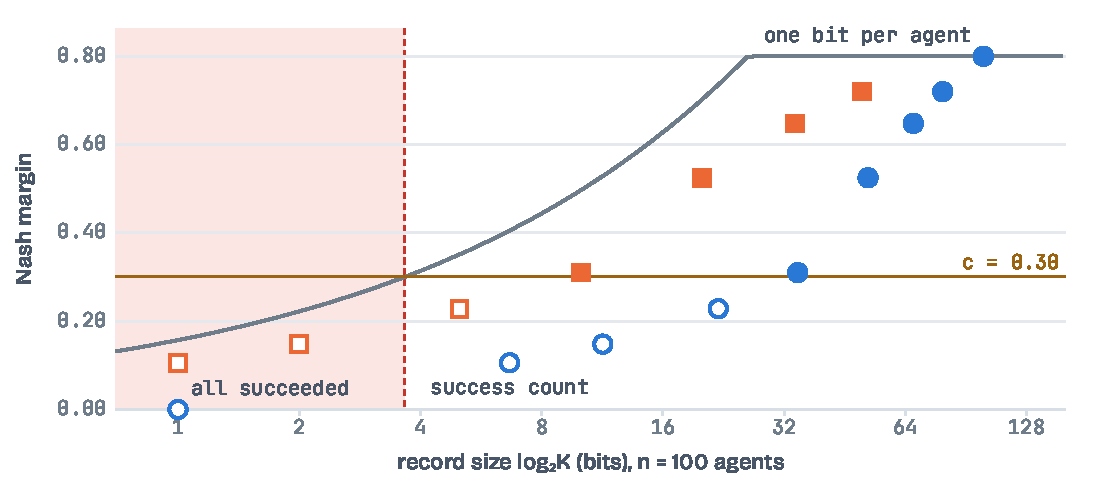
\includegraphics[width=\linewidth,page=1]{figures/g_memory.pdf}
\caption{Nash margin against record size, $n=100$.}\end{subfigure}\hfill
\begin{subfigure}[b]{0.44\textwidth}\centering
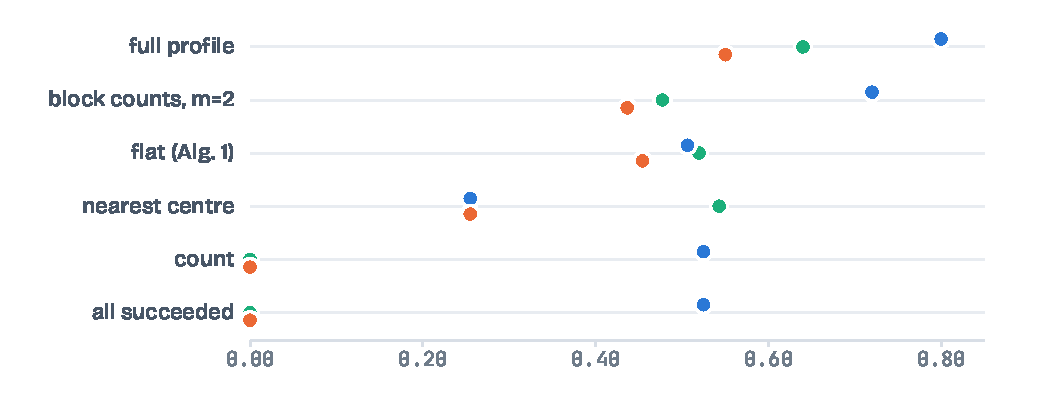
\includegraphics[width=\linewidth,page=1]{figures/g_attribution.pdf}
\caption{Detection against attribution, $n=5$.}\end{subfigure}
\caption{Noisy outcomes, $h=0.9$, $l=0.1$. (a) Exact Nash margins of block-count records
(circles) and of one threshold bit per block (squares, \cref{prop:blocks}), from one bit per
agent (right) to a single bit or the success count (left); the squares get the same margins
with far fewer bits; the grey curve bounds every record of that size (\cref{thm:noisy}), and
the shaded region is infeasible for every record at effort cost $c=0.3$ (amber line).
(b) Nash margin (blue), budget-balanced margin (orange) and the attribution bound of
\cref{thm:bb} (green) for each record; symmetric records detect but attribute nothing.}
\Description{Two charts. Left: Nash margin on the vertical axis against record size in bits on a logarithmic horizontal axis for 100 agents. Circles for block counts and squares for one threshold bit per block rise from near zero at one bit to 0.8 at 100 bits; the squares reach each margin with far fewer bits and lie close to a grey upper-bound curve; a shaded region on the left marks sizes that cannot sustain effort cost 0.3. Right: dot plot for six records showing Nash margin, budget-balanced margin and attribution bound; the count and all-succeeded records have zero budget-balanced margin and zero attribution bound.}
\label{fig:noisy}
\end{figure*}

\paragraph{The price in payments.} We now return to separately bounded payments, without
the fixed-total constraint. A record can sustain effort and still make it expensive.
Say a label \emph{certifies} agent $i$'s success if every profile that can produce it has
$S_i=1$.

\begin{proposition}[Cost of implementation]\label{prop:cost}
Let $0<c\le h-l$. For every record, the least expected payment making working a best
response for agent $i$ at cost $c$, when teammates work, is at least $ch/(h-l)$, the cost under the full record. It
equals $ch/(h-l)$ if and only if $c\le(h-l)\Pr[Y\text{ certifies }i\mid S_i=1]$.
\end{proposition}
\begin{proof}
For every label with $Q_1(y)>0$, $Q_{0,i}(y)/Q_1(y)$ is an average of the likelihood ratios $l/h$ and
$(1-l)/(1-h)$, so it is at least $l/h$, with equality exactly on certifying labels. Hence
$(h-l)Q_1(y)\ge h(Q_1(y)-Q_{0,i}(y))$ for every $y$, so any $p\in[0,1]^K$ with
$\langle p,Q_1-Q_{0,i}\rangle\ge c$ pays $\langle p,Q_1\rangle\ge ch/(h-l)$, with equality
only if $p$ lives on certifying labels, which carry total gain
$(h-l)\Pr[Y\text{ certifies }i\mid S_i=1]$.
\end{proof}

A count certifies agent $i$ only when everyone succeeded, with probability $h^{n-1}$, so it
leaves the floor once $c>(h-l)h^{n-1}$: at $c=0.02$ it costs 1.699 times the full record at
$n=100$ and 6.989 times at $n=1000$, and it cannot sustain $c=0.05$ at $n=1000$. The flat
record certifies nothing and pays a premium of 6 to 7\% at $n=5$ for its robustness.

\begin{proposition}[Memory is bought per accountable agent]\label{prop:designer}
Let $0<c\le h-l$ and $\beta=\beta(c)$ as in \cref{thm:tight}. A record of $\log_2K$
bits holds at most $\log_2K/\beta$ agents to cost $c$ and pays each at least $ch/(h-l)$;
recording each accountable agent's own outcome uses one bit per agent and attains that
payment. For the incentive-only objective, with no reconstruction constraint, suppose the principal
gains $v$ per working agent and pays $\kappa>0$ per bit of log-cardinality. Then
holding any agent to account is unprofitable when $v-ch/(h-l)<\kappa\beta$, holding all $n$
with $n$ bits is profitable when $v-ch/(h-l)>\kappa$, and any optimal record implementing a nonempty working set uses between $\beta$ and
1 bit per working agent.
\end{proposition}
\begin{proof}
The proof of \cref{thm:noisy} uses only independence of outcomes, so its bound holds at every
action profile, summed over the agents who work; this gives the capacity. The payment floor
is \cref{prop:cost}. For any selected working set, retaining its outcome bits attains
that floor; a record using more bits is strictly more expensive when $\kappa>0$.
\end{proof}

The designer jointly chooses the working set and its record. The bounds constrain memory
per incentivised agent; they do not solve the trade-off within the intermediate region.

%% =====================================================================
\section{Repeated Tasks and Deferred Settlement}\label{sec:repeated}
%% =====================================================================

Deployed agents handle many tasks, and repetition is the classical source of incentives that
a single signal cannot provide~\cite{radner1985repeated,jacksonsonnenschein2007}. We ask what
it changes for the memory of accountability. Each agent performs $T$ tasks with outcomes
$S_{i,t}$ distributed as in \cref{sec:noisy}, independently across agents and tasks; agent $i$
chooses an effort plan $a_i\in\cube^T$ at cost $c$ per worked task and observes no outcome
before settlement. Under \emph{per-task settlement}, task $t$ has its own record $Y_t$ of
$(S_{1,t},\dots,S_{n,t})$ and agent $i$ receives $p_{i,t}(Y_t)\in[0,1]$. Under \emph{deferred
settlement}, one record $Y$ encodes the whole history and agent $i$ receives
$P_i(Y)\in[0,T]$: the same aggregate payment cap per agent, paid once; expected payments need not be equal.

\begin{proposition}[Per-task settlement adds nothing]\label{prop:pertask}
Under per-task settlement the game is $T$ independent copies of the one-shot game: all-work at
cost $c$ is a Nash equilibrium only if $\sum_t\log_2K_t\ge Tn\,\beta(c)$, and no record
sustains any $c>h-l$.
\end{proposition}
\begin{proof}
Payoffs are additive, and the payment for task $t$ depends only on $Y_t$, hence only on
task-$t$ actions; apply \cref{cor:noisy}(i) to each task. A margin is a total variation
between label laws that are garblings of Bernoulli$(h)$ and Bernoulli$(l)$, so it is at most
$h-l$.
\end{proof}

\begin{theorem}[Deferred settlement]\label{thm:deferred}
(i) If all-work is a Nash equilibrium of the deferred game at cost $c$, then
$\log_2K\ge n\,\beta(c)/T$. (ii) A record symmetric in the agents admits no budget-balanced
deferred payment sustaining any $c>0$. (iii) The \emph{review record} keeps one bit per agent,
$b_i=\mathbf1\{\sum_tS_{i,t}>k\}$, and pays $P_i=T\,b_i$. Working on every task is strictly
dominant for every agent, so all-work is the unique equilibrium, if and only if $c<c_T(k)$,
where
\[ c_T(k)=\min_{1\le j\le T}\tfrac Tj\big(\pi_0-\pi_j\big),\quad
\pi_j=\Pr[\mathrm{Bin}(T{-}j,h)+\mathrm{Bin}(j,l)>k]. \]
\end{theorem}
\begin{proof}
(i) A deviation on a single task $(i,t)$ changes only the law of $S_{i,t}$, and since
$P_i/T\in[0,1]$, equilibrium needs the record's total variation under that deviation to be at
least $c/T$. The proof of \cref{thm:noisy} uses only independence of the outcomes, so it
applies to all $nT$ of them: $nT(c/T)^2\le\frac{(h-l)^2}{2h(1-h)}\ln K$. (ii) Apply the proof
of \cref{thm:bb} to the $n$ single-task deviations at one task, with payments scaled by
$1/T$; symmetry makes their label laws coincide. (iii) $P_i$ depends only on $i$'s own
outcomes, so $i$'s payoff does not depend on teammates' plans, and by exchangeability a plan
that shirks $j$ tasks earns $T\pi_j-c(T-j)$.
\end{proof}

\begin{table}[t]
\caption{Review records under deferred settlement, $h=0.9$, $l=0.1$: best threshold $k^*$ and
the largest cost $c_T(k^*)$ below which working is strictly dominant, against the per-task cap
$h-l=0.8$. Memory is one bit per agent for all $T$ tasks.}
\label{tab:review}
\footnotesize
\begin{tabular}{@{}lrrrrrr@{}}
\toprule
$T$ & 1 & 5 & 10 & 20 & 50 & 100\\
\midrule
$k^*$ & 0 & 3 & 7 & 15 & 40 & 83\\
$c_T(k^*)$ & 0.8000 & 0.9181 & 0.9298 & 0.9568 & 0.9755 & 0.9794\\
bits per agent per task & 1 & 0.2 & 0.1 & 0.05 & 0.02 & 0.01\\
\bottomrule
\end{tabular}
\end{table}

Within this no-feedback model, deferral improves achievable effort costs. Distinguishability among individual deviators is additionally necessary for positive incentives under a fixed total payment. As listed in \cref{tab:review}, one bit per agent sustains costs above $h-l$, which no
one-shot or per-task record can reach, whereas per-task settlement at $c=0.5$ needs at least
$0.10\,T$ bits per agent; this is the record-design counterpart of linking
decisions~\cite{jacksonsonnenschein2007} and review strategies~\cite{radner1985repeated}.
Part (ii) keeps symmetric records out, and part (i) keeps memory linear in $n$ for fixed $T$ and $c$; its coefficient decreases as $1/T$. The closed form
was checked against brute force over all $2^T$ effort plans for $T\le8$. Review records need
the absence of interim feedback: an agent that sees its outcomes before settlement can condition
effort on progress, the known weakness of review strategies~\cite{radner1985repeated}.

%% =====================================================================
\section{Exact Outcomes: When Is Accountability Free?}\label{sec:exact}

%% =====================================================================

We return to the exact model, in which the record observes the effort profile itself, and
ask what accountability costs in reconstruction error.

\subsection{One retained bit}\label{sec:onebit}

\begin{theorem}[One-bit frontier]\label{thm:onebit}
Let $n$ be odd, $S$ uniform and $K=2$, with arbitrary bounded payments and reconstruction.
Put $M_n=\E[\min(|S|,n-|S|)]$. Then for $0\le\mu\le1/n$,
\[ D^*(2,\mu)=M_n+n\mu\Big(\tfrac{n-1}{2}-M_n\Big), \]
and no record implements margin $\mu>1/n$, whatever the payment rule.
\end{theorem}

\begin{proof}
For $\mu=0$, the reconstruction-pair bound below gives $M_n$, attained by majority. Suppose $\mu>0$. \emph{Orientation.} The record is one function $q(s)=\Pr(Y=1\mid S=s)$ and
$d_i=(-\delta_i,\delta_i)$ with $\delta_i(s_{-i})=q(1,s_{-i})-q(0,s_{-i})$. Since
$|p_i[1]-p_i[0]|\le1$, \eqref{eq:M} holds iff some sign $\sigma_i$ has
$\sigma_i\delta_i(s_{-i})\ge\mu$ for all $s_{-i}$. \emph{Alignment.} Flipping the inputs and
the reconstruction on $T=\{i:\sigma_i=-1\}$ leaves $D$ unchanged under the uniform prior and
makes every $\sigma_i=+1$. Writing $q(s)=\mu|s|+r(s)$, the margin condition says exactly that
$r$ is monotone, and $q\in[0,1]$ gives $0\le r\le1-n\mu$, which is empty for $n\mu>1$.
\emph{Fix the reconstruction first.} Decode label 0 to $a$ and label 1 to $b$ and let
$\Delta(s)=\dH(s,b)-\dH(s,a)$. Since $\E[\dH(S,a)]=n/2$ for every $a$,
$D=\frac n2+\E[q(S)\Delta(S)]$, linear in $q$; under optimal decoding $D$ would be concave in
$q$, which is why the order matters. Using $0\le r\le1-n\mu$ pointwise,
$D\ge\frac n2+\mu\E[|S|\Delta(S)]-(1-n\mu)\E[\Delta(S)^-]$. \emph{Minimise over pairs.} If
$p$ and $m$ coordinates have $(a_i,b_i)=(0,1)$ and $(1,0)$, then
$\E[|S|\Delta]=-\frac12(p-m)\ge-\frac n2$ and $\E[\Delta^-]=\frac12\E|R_{p+m}|$ for a sum $R_k$
of $k$ independent Rademacher variables; $k\mapsto\E|R_k|$ is nondecreasing, so
$\E[\Delta^-]\le\frac n2-M_n$, which gives the lower bound. \emph{Attainment.} With
$(a,b)=(0^n,1^n)$, $\Delta(s)=n-2|s|$ and both inequalities are tight for
$r^*(s)=(1-n\mu)\mathbf1\{|s|>n/2\}$, an up-set indicator.
\end{proof}

The optimal record mixes a random-bit sampler with majority vote in proportion $n\mu$ to
$1-n\mu$ (\cref{fig:onebit}); an exhaustive LP over all reconstruction orbits matches the closed
form to within $3.1\times10^{-15}$ at $n=3,5,7,9$.

\begin{figure}[t]
\centering
\begin{subfigure}[b]{0.95\columnwidth}\centering
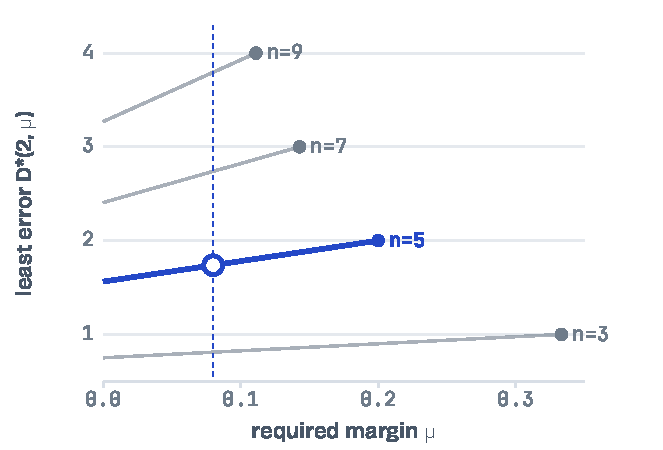
\includegraphics[width=\linewidth,page=1]{figures/g_onebit_frontier.pdf}
\caption{$D^*(2,\mu)$ for $n=3,5,7,9$.}\end{subfigure}
\begin{subfigure}[b]{0.95\columnwidth}\centering
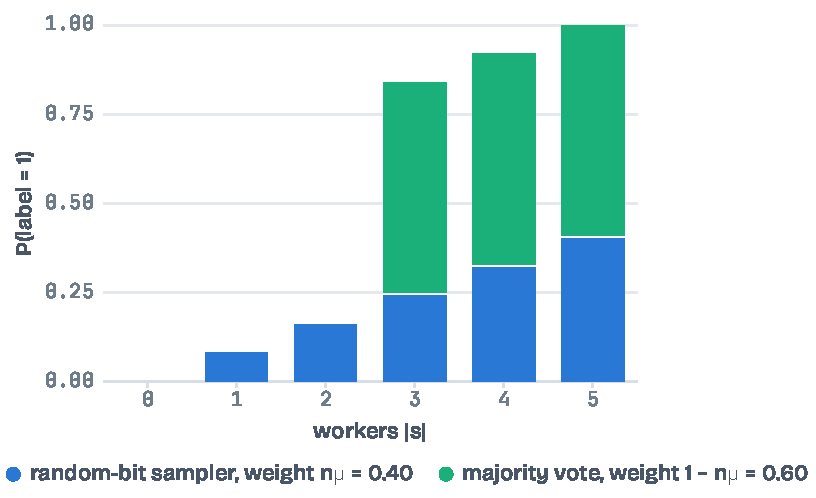
\includegraphics[width=\linewidth,page=1]{figures/g_onebit_record.pdf}
\caption{$q^*$ at $n=5$, $\mu=0.08$, by number of workers.}\end{subfigure}
\caption{The one-bit frontier (\cref{thm:onebit}). (a) Each line ends at $(1/n,(n-1)/2)$;
the open circle marks $\mu=0.08$ at $n=5$, where the least error rises from $M_5=1.5625$ to
$1.7375$. (b) The sampler adds exactly $\mu$ per worker; majority vote supplies the rest.}
\Description{Two charts. Top: least reconstruction error against required margin for 3, 5, 7 and 9 agents; each is a straight line ending at margin one over n, with a marked point at margin 0.08 for five agents. Bottom: stacked bars of the probability that the one-bit record outputs 1, by the number of agents who worked, split into a random-bit sampler part that grows linearly and a majority-vote part present only when most agents worked.}
\label{fig:onebit}
\end{figure}

\subsection{The flatness threshold}\label{sec:flat}

Call $C\subseteq\cube^n$ the \emph{centres} of a record, the reconstruction targets of its
$K$ labels.

\begin{lemma}[Necessity]\label{lem:nec}
Let $D_0$ be strictly decreasing at $K$, so the centres are distinct. If some non-centre $s$
has a unique nearest centre, the record is not flat, for any bounded payment.
\end{lemma}
\begin{proof}
Step from $s$ one bit towards its unique nearest centre $c$ to get $s'$; $c$ is still the
unique nearest centre of $s'$. Attaining $D_0(K)$ forces $q[s,\cdot]$ and $q[s',\cdot]$ to be
the point mass on $c$'s label, so that edge has $d_i=0$ and \cref{cor:edge} gives margin 0.
\end{proof}

When $C$ is dominating, \cref{lem:nec} requires every vertex outside $C$ to have at least two
neighbours in $C$: $C$ is a \emph{2-dominating set} of the hypercube $Q_n$. The converse holds
constructively.

\begin{lemma}[Sufficiency]\label{lem:suff}
Let $C$ be 2-dominating with $|C|=K<2^n$. The record that maps each centre to its own label and
each other profile uniformly to the labels of its neighbouring centres, decoded to the centre
and paying agent $i$ the $i$-th bit of the centre, has $D=D_0(K)=(2^n-K)/2^n$ and margin
$1-1/\dmin\ge1/2$, where $\dmin=\min_{t\notin C}|N(t)\cap C|$.
\end{lemma}
\begin{proof}
\emph{Error.} Centres are reconstructed exactly and every other profile costs one bit; any
$K$-label record reconstructs at most $K$ profiles exactly, so $D_0(K)\ge(2^n-K)/2^n$.
\emph{Margin.} Let $d(t)=|N(t)\cap C|$. On an edge $s_1=s_0+e_i$: if both ends are centres the
gap is 1; if only $s_1$ is, the centre-neighbours of $s_0$ are $s_1$ and vertices $s_0+e_j$
with bit $i$ equal to 0, so the gap is $1-1/d(s_0)$; the reverse case is symmetric; if
neither is, every centre-neighbour of $s_1$ has bit $i$ equal to 1 and every one of $s_0$ has
it 0, so the gap is 1.
\end{proof}

\begin{theorem}[Flatness in the dominating-code regime]\label{thm:flat}
Under the uniform prior, for $\gamma(Q_n)\le K\le2^n$, a flat record of size $K$ exists
if and only if $K\ge\gamma_2(Q_n)$. In particular,
$\Kflat(n)\le\gamma_2(Q_n)$ for every $n$. For a proper 2-dominating code, the construction
in \cref{lem:suff} has margin at least $1/2$; the full code has margin 1.
\end{theorem}
\begin{proof}
For $K\ge\gamma(Q_n)$ a dominating code attains $D_0(K)=(2^n-K)/2^n$.
Any optimal code must then be dominating: a non-centre at distance at least 2 would
strictly increase this sum. By \cref{lem:nec}, a flat optimal code is 2-dominating.
Conversely, enlarge a minimum 2-dominating code to size $K$; 2-domination is preserved,
and \cref{lem:suff} applies (or use the full record when $K=2^n$).
\end{proof}

Equality $\Kflat(n)=\gamma_2(Q_n)$ requires excluding flat codes below $\gamma(Q_n)$.
The following necessary condition supports finite-dimensional exclusions; no general
exclusion below that regime is claimed.

\begin{lemma}[Shell bound]\label{lem:shell}
In a flat record, for each $r\ge1$, every profile at distance $r$ from $C$ has at least two centres at distance
$r$, so shell $r$ holds at most $\lfloor K\binom nr/2\rfloor$ profiles, and filling shells from
the inside lower-bounds $2^nD_0(K)=\sum_sd(s,C)$.
\end{lemma}
\begin{proof}
A unique nearest centre at radius $r$ yields a zero-margin edge as in \cref{lem:nec}. Each
centre is at distance $r$ from $\binom nr$ profiles, and each profile in shell $r$ uses two
of the at most $K\binom nr$ (profile, centre) pairs.
\end{proof}

In shell 1 this gives Fink and Jacobson's bound
$\gamma_k(G)\ge k|V|/(\Delta+k)$~\cite{fink1985ndomination}. Combined with known
domination numbers~\cite{ostergard2001length9}, explicit codes, and the supplement's
certificate chain, the exclusions give $\Kflat(3)=4$, $\Kflat(5)=10$,
$\Kflat(7)=32$, and $\Kflat(9)\in[97,128]$. The $n=9$ threshold remains open.
For general $n$, the bounds
$2^{n+1}/(n+2)\le\gamma_2(Q_n)\le2^{n-\lfloor\log_2(n/2+1)\rfloor}$
describe the 2-dominating construction, not an unconditional lower bound on $\Kflat(n)$.
For example, this construction retains 17 bits at $n=20$.



\begin{figure*}[t]
\centering
\begin{subfigure}[b]{0.3\textwidth}\centering
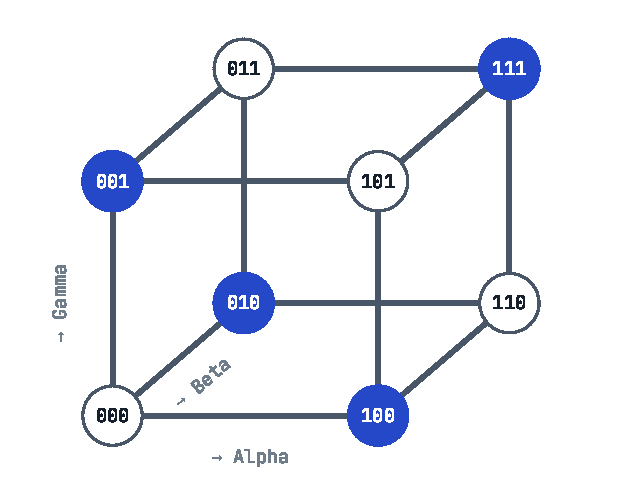
\includegraphics[width=\linewidth,page=1]{figures/g_cube_flat.pdf}
\caption{Flat: $D=0.5$, $\mu=2/3$.}\end{subfigure}\hfill
\begin{subfigure}[b]{0.3\textwidth}\centering
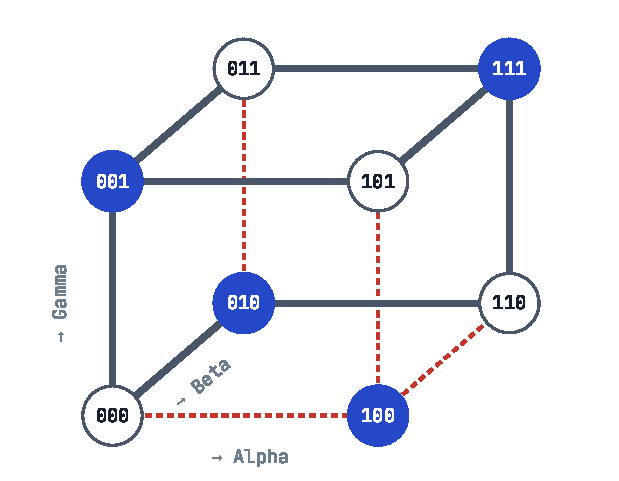
\includegraphics[width=\linewidth,page=1]{figures/g_cube_near.pdf}
\caption{Nearest centre: $D=0.5$, $\mu=0$.}\end{subfigure}\hfill
\begin{subfigure}[b]{0.3\textwidth}\centering
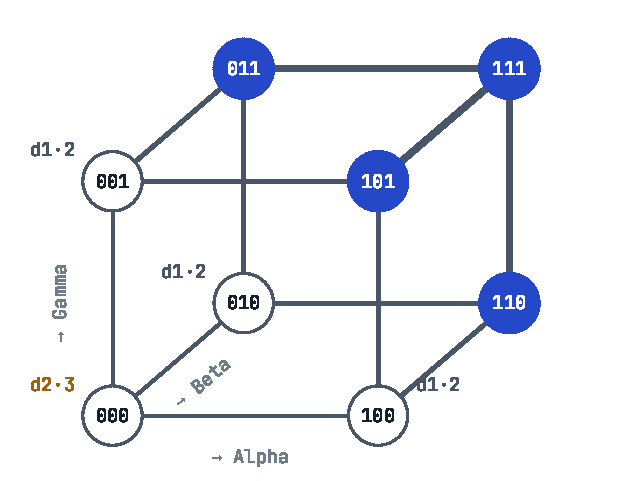
\includegraphics[width=\linewidth,page=1]{figures/g_cube_prior.pdf}
\caption{Bernoulli$(0.7)$ prior: flat, $\mu=1/3$.}\end{subfigure}
\caption{Records on the 3-cube. Filled vertices are centres; edge width denotes total
variation. (a) Uniformly choosing a neighbouring centre is flat. (b) Deterministic nearest-centre
assignment has the same error but zero margin: three edges are dead (red).
(c) Under a Bernoulli$(0.7)$ prior, an optimal code is flat without being 2-dominating
(Theorem S1): $000$ has three nearest centres at distance 2.}
\Description{Three drawings of the 3-dimensional cube of effort profiles. Left: four filled centres forming the odd-weight class, all edges solid. Middle: the same centres with each other profile sent to one nearest centre; three edges are red and dashed, meaning one agent changing its effort leaves the record unchanged. Right: a different set of four centres for a tilted prior; profile 000 is at distance two from three centres, yet every edge is solid.}
\label{fig:cubes}
\end{figure*}

\paragraph{Other priors.} \eqref{eq:M} never mentions the prior, and \cref{lem:nec} survives
for any full-support prior at whatever radius the nearest centre lies. The supplement
(Theorem S1) shows that the threshold is the least $K$ for which some prior-optimal code gives
every non-centre at least two nearest centres; tilting moves it either way (7 at $n=4$ under
the uniform prior, 5 when each agent works with probability $0.7$, 13 at $0.6$), and
\cref{fig:cubes}(c) shows a flat record that is not 2-dominating.

%% =====================================================================
\section{Measured Mechanisms}\label{sec:experiments}
%% =====================================================================

We evaluate stylised count, threshold, prefix, hash and nearest-centre records by enumerating
all profiles and solving the margin LP. These finite-model calculations are separate from
the sampled language-model study below. The supplement reports the registered conjectures,
including failures, and the reproducibility checks.

\paragraph{Compaction mechanisms.} As listed in \cref{tab:mech}, no mechanism beats the
frontier, and at this $n=5$ none below the certified threshold $K=10$ is flat. The last two rows use the same ten labels
and have the same error $D_0(10)=0.6875$; one admits margin $1/2$ and the other none, for any
bounded decoder, so a designer comparing records on reconstruction alone cannot see the
difference. Keeping the first $m$ agents' bits gives margin exactly 0 for every $m<n$: prefix-4
is reconstruction-optimal at its budget and worthless for accountability.

\begin{table}[t]
\caption{Compaction mechanisms at $n=5$, uniform prior, no noise. Flat: $D=D_0(K)$ and $\mu>0$.}
\label{tab:mech}
\footnotesize
\begin{tabular}{@{}lrrrrl@{}}
\toprule
mechanism & $K$ & $D$ & $D_0(K)$ & $\mu$ & flat\\
\midrule
full profile & 32 & 0.0000 & 0.0000 & 1.0000 & yes\\
count & 6 & 1.5625 & 0.8750 & 0.2000 & no\\
threshold & 2 & 1.5625 & 1.5625 & 0.0000 & no\\
prefix-4 & 16 & 0.5000 & 0.5000 & 0.0000 & no\\
top-2 & 16 & 0.7188 & 0.5000 & 0.0000 & no\\
hash-10 & 10 & 1.5000 & 0.6875 & 0.0000 & no\\
\midrule
flat (\cref{lem:suff}) & 10 & 0.6875 & 0.6875 & 0.5000 & \textbf{yes}\\
$K$-median & 10 & 0.6875 & 0.6875 & 0.0000 & no\\
\bottomrule
\end{tabular}
\end{table}

\paragraph{Episodes.} When agents return artifacts and a record compresses the whole trace, at
$n=5$ the full trace and one bit per agent keep margin $0.5000$, while the multiset of artifacts,
which loses only authorship, keeps $0.1425$.

\paragraph{Model-written reviews: an attribution illustration.}
The saved codestral-2508 study uses 192 episodes, one fixed diff and three reviewer roles.
``Effort'' is assigned by supplying the diff or requesting generic guidance without it;
no strategic response is measured. The same model judges retained records at temperature 0.
Removing names \emph{and shuffling order} retains identical review text and saves 30 bytes
on average, but raises mean Hamming error from 0.391 to 1.333 wrong agent labels out of three
(paired difference 0.943; episode-bootstrap 95\% CI $[0.802,1.089]$).
The comparison combines both transformations. Specialised content may reveal identity,
so it does not establish the symmetry required by \cref{cor:bb}. Fixed roles, one diff and
a shared generator/judge limit generalisability. The supplement reports all conditions,
metric definitions and finite-sample limitations.

%% =====================================================================
\section{Related Work}\label{sec:related}
%% =====================================================================

\paragraph{Contracts and information.}
Jewitt, Kadan and Swinkels~\cite{kadanswinkels2008} study bounded-payment moral hazard;
Georgiadis and Szentes~\cite{georgiadisszentes2020} design monitoring for one agent.
We constrain a shared retained alphabet serving multiple agents' incentives and reconstruction.
The minimax/total-variation tools are standard, with signal comparisons and informativeness
as background~\cite{blackwell1953comparisons,holmstrom1979moral}.
Unlike persuasion~\cite{kamenica2011persuasion}, our signal supports hidden-action incentives.

\paragraph{Teams, repetition and communication.}
Team moral hazard~\cite{holmstrom1982teams,legrosmatthews1993,rahmanobara2010} motivates
fixed-total payments; \cref{thm:bb} quantifies attribution among deviators.
Repetition~\cite{radner1985repeated,jacksonsonnenschein2007} already relaxes incentives;
we bound retained memory and give a finite-horizon threshold without interim feedback.
Communication models~\cite{fadelsegal2009,blumrosen2007auctions} address hidden types;
our evidence concerns hidden actions. Learning-agent contracts~\cite{haupt2023contracts,ivanov2024principal,shao2025truth}
and cooperative credit assignment~\cite{foerster2018coma,sunehag2018vdn,rashid2018qmix,li2025nucleolus}
address related questions. Attribution accuracy alone does not establish implementable incentives.
The 2-domination invariant is classical~\cite{fink1985ndomination,chellali2012survey,bujtas2016bounds,ostergard2001length9};
we connect it to reconstruction-optimal records in the specified regime.

%% =====================================================================
\section{Conclusion}\label{sec:conclusion}
%% =====================================================================

For independent noisy outcomes, fixed-cost Nash incentives require linear memory in
team size; threshold blocks attain the same order. Fixed-total payments additionally
require distinguishable individual deviators. For exact outcomes, 2-dominating codes
combine optimal reconstruction with positive dominant-strategy incentives. Designers
should therefore test incentive margins separately from reconstruction error and specify
what evidence settlement can retain. Names are one way to preserve attribution;
threshold bits and deferred review provide other savings under their stated assumptions.

\paragraph{Limitations and outlook.}
We assume binary costly actions, commitment, and no settlement evidence outside the record.
The noisy bound uses independent outcomes and fixed $h,l$; reconstruction uses Hamming loss.
Repetition excludes interim feedback and counts terminal records, not online working memory.
A strategic compactor needs separate incentives to implement the desired channel.
Open problems include correlated or heterogeneous outcomes, excluding flat codes below the
domination regime, resolving $\Kflat(9)\in[97,128]$, and closing the asymptotic memory gap.
Controlled multi-task experiments are needed for LLM deployment claims.

\label{endbody}\clearpage
\balance
\bibliographystyle{ACM-Reference-Format}
\bibliography{refs}

\end{document}

